\documentclass{article}
\usepackage[margin=1in]{geometry}
\usepackage{graphicx}
\pagestyle{empty}
\usepackage{floatrow}
\usepackage{subfig}
\captionsetup[subfigure]{labelformat=simple,position=top,justification=justified,singlelinecheck=false}
\captionsetup[figure]{labelformat=simple,labelsep=space,labelfont=bf}

\title{ataqv manuscript figures}

\begin{document}

\floatsetup[figure]{style=plain,subcapbesideposition=top}

\maketitle
\pagestyle{empty}

  
\renewcommand{\thefigure}{\textbf{\arabic{figure}. }}
\setcounter{figure}{0}

\begin{figure}
\includegraphics[width=\textwidth,trim=0em 2em 0em 0em,clip=true]{public_fig}
\caption{}
\end{figure}


\begin{figure}
\includegraphics[width=\textwidth]{tn5_fig}
\caption{}
\end{figure}


%%%%%%%%%%%%%%%%%%%%%%%%
  %%%% Supplemental figures
%%%%%%%%%%%%%%%%%%%%%%%%
\renewcommand{\thefigure}{\textbf{S\arabic{figure}. }}
\setcounter{figure}{0}

\begin{figure}
\subfloat[]{\includegraphics[width=0.9\textwidth,trim=0em 25em 0em 25em,clip=true]{ataqv-workflow}}\\
\subfloat[]{\includegraphics[width=\textwidth]{ataqv_screenshot}}
\caption{}
\end{figure}

\begin{figure}
	\subfloat[]{\includegraphics[width=0.5\textwidth]{example_fld_calculation_density}}
	\subfloat[]{\includegraphics[width=0.5\textwidth]{example_fld_calculation_cumulative}}
\caption{}
\end{figure}


\begin{figure}
\subfloat[]{\includegraphics[width=0.5\textwidth]{public_intrastudy_heterogeneity_fragment_length_distributions}}
\subfloat[]{\includegraphics[width=0.5\textwidth]{public_intrastudy_heterogeneity_tss_enrichment}}\\
\caption{}
\end{figure}

\begin{figure}
	\subfloat[]{\includegraphics[width=0.7\textwidth]{public-bulk-hg19-max-fraction}}\\
	\subfloat[]{\includegraphics[width=0.7\textwidth]{public-bulk-mm9-max-fraction}}
	\caption{}
\end{figure}

\begin{figure}
	\includegraphics[width=0.5\textwidth]{{PRJNA259243-hg19.tss_enrichment_scatter}.pdf}
	\caption{}
\end{figure}

\begin{figure}
	\subfloat[]{\includegraphics[width=0.5\textwidth]{su_et_al_median_fragment_length_vs_batch}}\\
	\subfloat[]{\includegraphics[width=0.5\textwidth]{su-et-al-qqplot}}
\caption{}
\end{figure}


\begin{figure}
	\subfloat[]{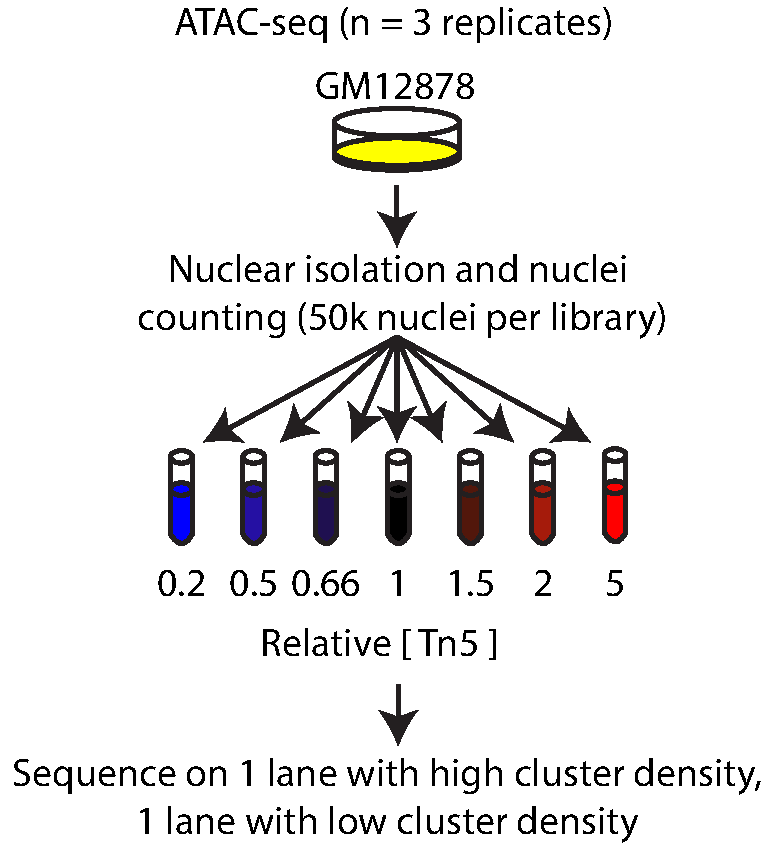
\includegraphics[width=0.25\textwidth]{cd_cartoon}}
	\subfloat[]{\includegraphics[width=0.35\textwidth]{cd_high_vs_low_median_fragment_length}}
	\subfloat[]{\includegraphics[width=0.35\textwidth]{cd_high_vs_low_tss_enrichment}}
\caption{}
\end{figure}

\begin{figure}
\includegraphics[width=\textwidth]{cd_pcr_cycles}
\caption{}
\end{figure}

\begin{figure}
	\includegraphics[width=\textwidth]{tn5_qpcr}
\caption{}
\end{figure}

\begin{figure}
\subfloat[]{\includegraphics[width=0.4\textwidth]{tn5_median_fragment_length_all_six}}
\subfloat[]{\includegraphics[width=0.4\textwidth]{tn5_mitochondrial_percent}}\\
\subfloat[]{\includegraphics[width=0.4\textwidth]{tn5_tss_enrichment_all_six}}
\subfloat[]{\includegraphics[width=0.4\textwidth]{tn5_proportion_duplicate}}\\
\subfloat[]{\includegraphics[width=0.4\textwidth]{tn5_proportion_hqaa}}
\caption{}
\end{figure}

\begin{figure}
\subfloat[]{\includegraphics[width=0.4\textwidth]{cd_median_fragment_length}}
\subfloat[]{\includegraphics[width=0.4\textwidth]{cd_mitochondrial_percent}}\\
\subfloat[]{\includegraphics[width=0.4\textwidth]{cd_tss_enrichment}}
\subfloat[]{\includegraphics[width=0.4\textwidth]{cd_hqaa_overlapping_peaks_percent}}\\
\subfloat[]{\includegraphics[width=0.4\textwidth]{cd_proportion_duplicate}}
\subfloat[]{\includegraphics[width=0.4\textwidth]{cd_proportion_hqaa}}
\caption{}
\end{figure}

\begin{figure}
\subfloat[]{\includegraphics[width=0.4\textwidth]{pcr-constant-number-of-peaks}}
\subfloat[]{\includegraphics[width=0.4\textwidth]{pcr-constant-number-of-peaks-after-subsampling-bams}}
\caption{}
\end{figure}

\begin{figure}
\subfloat[]{\includegraphics[width=0.4\textwidth]{pcr-constant-pairwise-peak-jaccard}}
\subfloat[]{\includegraphics[width=0.4\textwidth]{pcr-constant-pairwise-peak-jaccard-after-subsampling-bams}}
\caption{}
\end{figure}

\begin{figure}
\includegraphics[width=\textwidth]{tn5_pca}
\caption{}
\end{figure}

\begin{figure}
\includegraphics[width=\textwidth]{tn5_modeling}
\caption{}
\end{figure}

\begin{figure}
\includegraphics[height=5cm]{chromatin_state_legend}\\
\vspace{1cm}
\subfloat[]{\includegraphics[height=5cm]{promoter_rep1}}\hspace{0.25cm}
\subfloat[]{\includegraphics[height=5cm,trim=25em 0em 0em 0em,clip=true]{promoter_rep2}}\hspace{0.25cm}
\subfloat[]{\includegraphics[height=5cm,trim=25em 0em 0em 0em,clip=true]{promoter_rep3}}\\
\subfloat[]{\includegraphics[height=5cm]{promoter_rep4}}\hspace{0.25cm}
\subfloat[]{\includegraphics[height=5cm,trim=25em 0em 0em 0em,clip=true]{promoter_rep5}}\hspace{0.25cm}
\subfloat[]{\includegraphics[height=5cm,trim=25em 0em 0em 0em,clip=true]{promoter_rep6}}
\caption{}
\end{figure}

\begin{figure}
\includegraphics[height=5cm]{chromatin_state_legend}\\
\vspace{1cm}
\subfloat[]{\includegraphics[height=5cm]{enhancer_rep1}}\hspace{0.25cm}
\subfloat[]{\includegraphics[height=5cm,trim=25em 0em 0em 0em,clip=true]{enhancer_rep2}}\hspace{0.25cm}
\subfloat[]{\includegraphics[height=5cm,trim=25em 0em 0em 0em,clip=true]{enhancer_rep3}}\\
\subfloat[]{\includegraphics[height=5cm]{enhancer_rep4}}\hspace{0.25cm}
\subfloat[]{\includegraphics[height=5cm,trim=25em 0em 0em 0em,clip=true]{enhancer_rep5}}\hspace{0.25cm}
\subfloat[]{\includegraphics[height=5cm,trim=25em 0em 0em 0em,clip=true]{enhancer_rep6}}
\caption{}
\end{figure}

\begin{figure}
\includegraphics[height=5cm]{chromatin_state_legend}\\
\vspace{1cm}
\subfloat[]{\includegraphics[height=5cm]{insensitive_rep1}}\hspace{0.25cm}
\subfloat[]{\includegraphics[height=5cm,trim=25em 0em 0em 0em,clip=true]{insensitive_rep2}}\hspace{0.25cm}
\subfloat[]{\includegraphics[height=5cm,trim=25em 0em 0em 0em,clip=true]{insensitive_rep3}}\\
\subfloat[]{\includegraphics[height=5cm]{insensitive_rep4}}\hspace{0.25cm}
\subfloat[]{\includegraphics[height=5cm,trim=25em 0em 0em 0em,clip=true]{insensitive_rep5}}\hspace{0.25cm}
\subfloat[]{\includegraphics[height=5cm,trim=25em 0em 0em 0em,clip=true]{insensitive_rep6}}
\caption{}
\end{figure}

\begin{figure}
\includegraphics[width=\textwidth]{cd_modeling}
\caption{}
\end{figure}

\begin{figure}
\includegraphics[width=\textwidth]{cd_chromatin_state_overlap}
\caption{}
\end{figure}


\begin{figure}
\includegraphics[width=\textwidth]{tn5_tf_overlap}
\caption{}
\end{figure}

\begin{figure}
\includegraphics[width=\textwidth]{tn5_sensitivity_prob_by_chipseq_overlap_and_peak_signal}
\caption{}
\end{figure}

\begin{figure}
\includegraphics[width=0.4\textwidth]{nuclear_isolation_efficiency}
\caption{}
\end{figure}


\begin{figure}
\subfloat[]{\includegraphics[width=0.9\textwidth]{tss_coverage_different_methods}}\\
\subfloat[]{\includegraphics[width=0.5\textwidth]{tss_coverage_positional_stability}}
\caption{}
\end{figure}


\begin{figure}
\includegraphics[width=0.5\textwidth]{tss_enrichment_housekeeping_vs_all}
\caption{}
\end{figure}

\end{document}
